\documentclass[12pt, a4paper]{article}
\title{Эффект Холла в полупроводниках (3.3.4)}
\author{Стеценко Георгий, Б02-312}
\date{}
% !TeX encoding = UTF-8

\usepackage{geometry}
\usepackage{amsmath, amsfonts, amssymb, amsthm} % стандартный набор AMS-пакетов для математ. текстов
\usepackage{mathtext}
\usepackage[utf8]{inputenc} % кодировка utf8
\usepackage[russian]{babel} % русский язык
\usepackage[pdftex,dvipsnames]{xcolor} % работа с цветами
\usepackage[pdftex]{graphicx} % графика (картинки)
\usepackage{tikz,pgfplots} % рисунки
\usepackage{indentfirst}
%\usepackage[labelfont=bf,labelsep=endash,skip=3pt]{caption} % подпись картинок
% \usepackage{fancyhdr,pageslts} % настройка колонтитулов
\usepackage{enumitem} % работа со списками
\usepackage{floatrow,multicol,multirow,longtable,hhline} % работа с таблицами
\usepackage{float,wrapfig} % плавающие объекты
\usepackage{tcolorbox} % рамка вокруг текста
%\usepackage[calc]{datetime2} % дата
\usepackage{bm} % жирное начертание в формулах
\usepackage{physics} % физический пакет
\DeclareMathAlphabet\mathbfcal{OMS}{cmsy}{b}{n}
\usepackage{pgfornament} % красивые рюшечки и вензеля
\usepackage{mdframed}
\usepackage{derivative}
\usepackage{mathrsfs} %EDS
\usepackage{soul} % strikethorugh
%\usepackage{boondox-cal}

% ----------------------------------------
% Настройка шрифта

% Просто закооментируйте следующую строчку, если не работает. Будет другой шрифт, правда :(
% \usepackage{pscyr}

% ----------------------------------------
% Стилевые настройки

\usepackage{boldline} % жирная линия после таблиц (чтобы не было ошибок, этот пакет должен подключаться именно тут!)
\floatsetup[table]{style=Plaintop,floatrowsep=qquad} % настройка оформления таблиц
\setlist[enumerate,itemize]{leftmargin=5mm,itemindent=10mm,itemsep=0mm,
listparindent=0em,labelsep=2mm,topsep=2mm,labelwidth=4mm} % настройки списков

\setlength{\columnsep}{0.5cm} % расстояние между колонками
\setlength{\parskip}{1pt} % расстояние до текста от колонтитула

%\usepackage{titlesec} % управление оформлением section
%\renewcommand{\thesection}{\Roman{section}}
%\titleformat{\section}[block]{\bfseries\large}{\thesection.}{5pt}{}

% ----------------------------------------
% Настройки полей
\geometry{
  left=10mm,
  top=10mm,
  right=10mm,
  bottom=15mm,
  marginparsep=0mm,
  marginparwidth=0mm,
  headheight=0pt,
  headsep=0pt,
footskip=20pt}

% ----------------------------------------
% Настройки колонтитулов и нумерации страниц
\pagenumbering{arabic}



\newcounter{ntask}
\setcounter{ntask}{0}


\newcommand{\arsh}{\mathrm{arsh} \,\,}
\newcommand{\arch}{\mathrm{arch} \,\,}
\newcommand{\arth}{\mathrm{arth} \,\,}
\newcommand{\arcth}{\mathrm{arcth} \,\,}
\renewcommand{\Re}{\operatorname{Re} \,}
\newcommand{\EDS}{\mathscr{E}}
\newcommand{\diffract}[1]{\frac{\mathrm{d}#1}{\mathrm{d}t}}



\newcommand{\V}{~\mathrm{V}}
\newcommand{\mV}{~\mathrm{mV}}
\newcommand{\A}{~\mathrm{A}}
\newcommand{\mA}{~\mathrm{mA}}
\newcommand{\uT}{~\mathrm{\mu T}}
\newcommand{\mT}{~\mathrm{mT}}
\newcommand{\kHz}{~\mathrm{kHz}}
\newcommand{\Hz}{~\mathrm{Hz}}
\newcommand{\mm}{~\mathrm{mm}}

\addto\captionsrussian{\def\refname{Источники}}

\begin{document}
\maketitle

\section{Цель работы}
Измерение подвижности и концентрации носителей заряда в полупроводниках.


\section{Теоретические сведения}


\subsection*{Эффект Холла}

Во внешнем магнитном поле $\vec{B}$ на заряды действует сила Лоренца $\vec{F}=q\vec{E}+q\vec{u}\times\vec{B}$. Эта сила вызывает движение носителей, направление которого в общем случае не совпадает с $\vec{E}$. Возникновение попречного току электрического поля в образце, помещённом во внешнее магнитное поле, называют \textit{эффектом Холла}.

\subsection*{Мостик Холла}

\begin{wrapfigure}[12]{r}{0.4\textwidth}
  \centering
  \vspace{-15mm}
  \begin{center}
    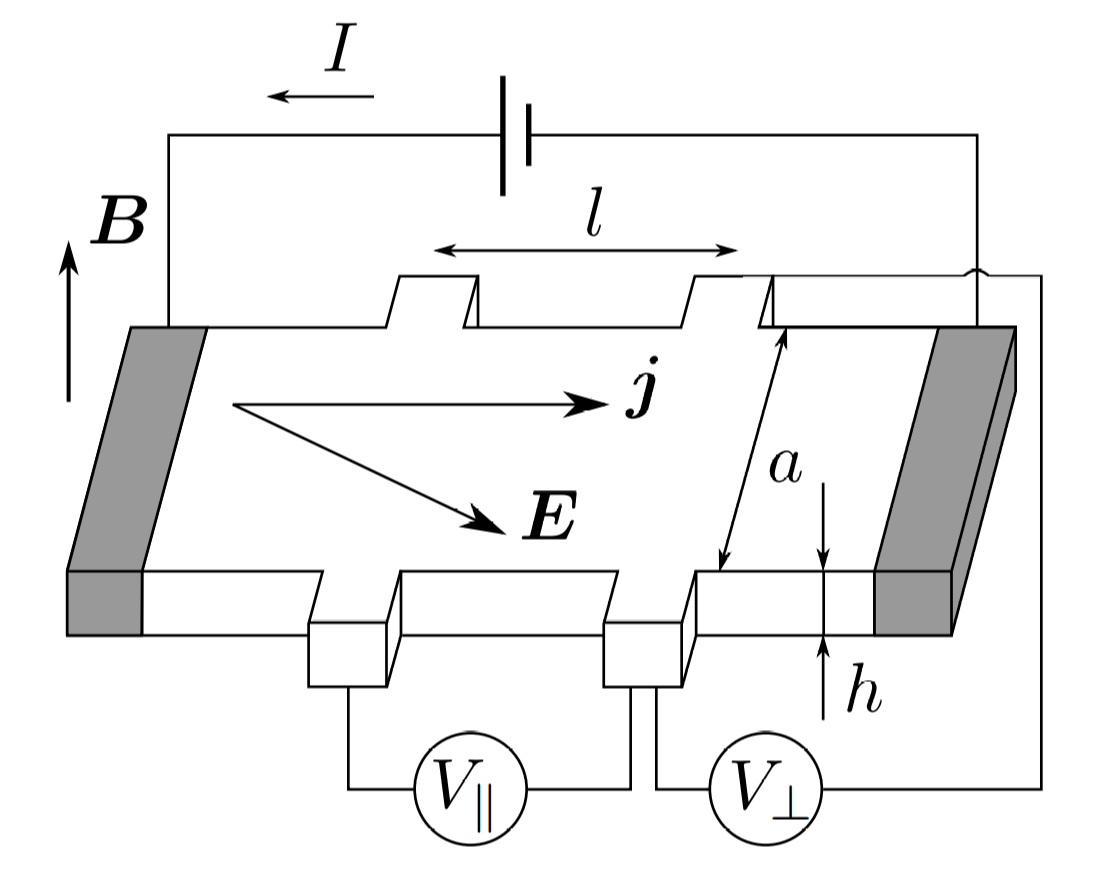
\includegraphics[width=0.95\textwidth]{pics/th}
  \end{center}
  \caption{Схема мостика Холла}\label{fig:th}
\end{wrapfigure}

Для исследования завиисимости проводимости среды от магнитного поля используют т.н. \textit{мостик Холла}. В данной схеме (см. рисунок \ref{th}) ток вынуждают течь по оси $x$ вдоль плоской пластинки (ширина пластинки $a$, толщина $h$, длина $l$). Сила Лоренца, действующая со стороны перпендикулярного пластинке магнитного поля, "прибивает" носители заряда к краям образца, что создаёт холловское электрическое поле, компенсирующее эту силу. Поперечное напряжение между краями пластинки (\textit{холловское напряжение}) равно $U_{\perp}=E_ya$, где\[E_y=\frac{j_xB}{nq}.\]Плотность тока, текущего через образец, равна $j_x=\frac{I}{ah}$, где $I$ -- полный ток, $ah$ -- поперечное сечение. Таким образом, для холловского напряжения имеем
\begin{equation}U_{\perp}=\frac{B}{nqh}I=R_H\frac{B}{h}I,\label{eq:uperp}
\end{equation}
где константу
\begin{equation}R_H=\frac{1}{nq}\label{eq:r_hall}
\end{equation}
называют \textit{постоянной Холла}. Знак постоянной Холла определяется знаком заряда носителей.

Продольная напряжённость электрического поля равна
\begin{equation}
  E_x=\frac{j_x}{\sigma_0},
  \label{eq:ey}
\end{equation}
и падение напряжения $U_{\parallel}=E_xl$ \textit{вдоль} пластинки определяется омическим сопротивлением образца $R_0=\frac{l}{\sigma_0ah}$:\[U_{\parallel}=IR_0.\]Интересно отметить, что немотря на то, что тензор проводимости явно зависит от $B$, продольное сопротивление образца в данной геометрии от магнитного поля \textit{не зависит}.


\section{Методика измерений}
\textbf{В работе используются:}  электромагнит с регулируемым источником пи­тания; вольтметр; амперметр; миллиамперметр; милливеберметр или мил­литесламетр; источник питания (1,5$\V$), образцы легированного германия.

\begin{wrapfigure}[21]{l}{0.5\textwidth}
  \centering
  \vspace{-8mm}
  \begin{center}
    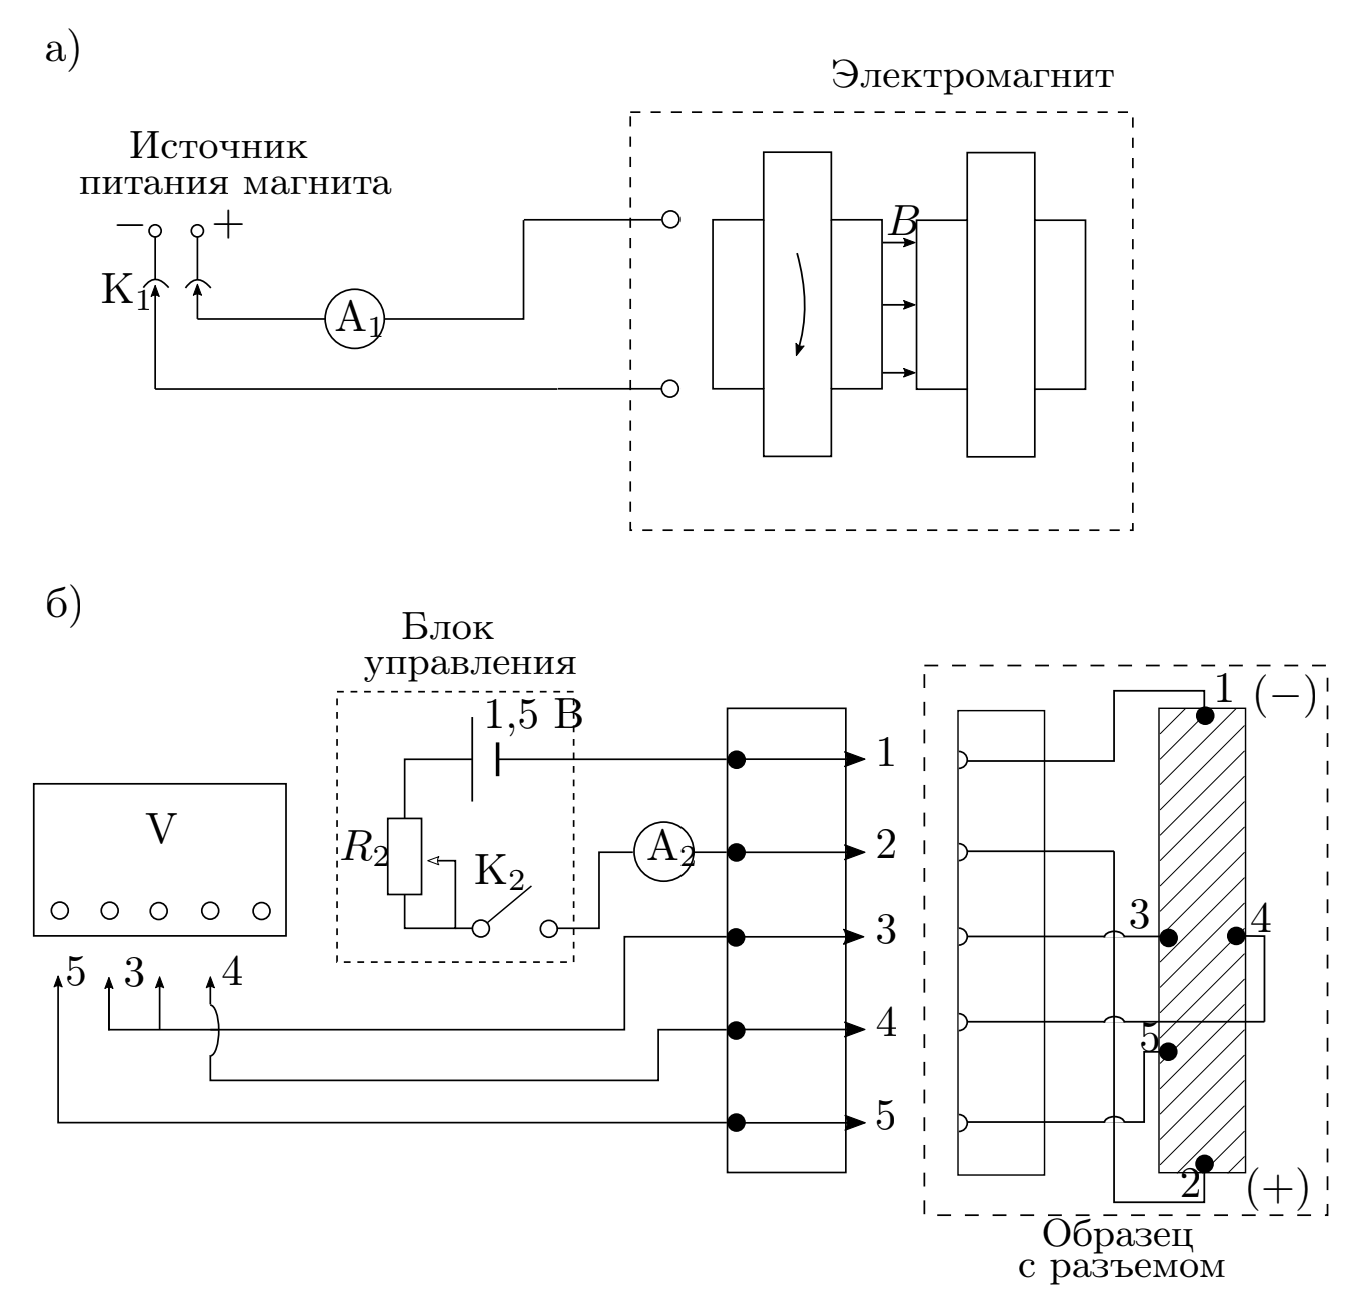
\includegraphics[width=0.95\textwidth]{pics/setup}
  \end{center}
  \caption{Установка}\label{fig:setup}
\end{wrapfigure}
В зазоре электромагнита создаётся постоянное магнитное поле, величину которого можно менять с помощью регуляторов источника питания.

Градуировка магнита проводится при помощи тесламетра, помещаемого напрямую в зазор электромагнита.

Образец из легированного германия, смонтированный в специальном держателе, подключается к батарее ($\approx1,5~\text{В}$). При замыкании ключа $K_2$ вдоль длинной стороны образца течёт ток, величина которого регулируется реостатом $R$ и измеряется миллиамперметром $A_2$.

В образце с током, помещённом в зазор электромагнита, между контактами 3 и 4 возникает разность потенциалов $U_{34}$, которая измеряется с помощью цифрового вольтметра.

Контакты 3 и 4 вследствие неточности подпайки не всегда лежат на одной эквипотенциали, и тогда напряжение между ними связано не только с эффектом Холла, но и с омическим падением напряжения, вызванным протеканием основного тока через образец. Измеряемая разность потенциалов при одном направлении магнитного поля равна сумме ЭДС Холла и омического падения напряжения, а при другом -- их разности. В этом случае ЭДС Холла $U_\perp$ может быть определена как половина алгебраической разности показаний вольтметра, полученных для двух противоположных направлений магнитного поля в зазоре. Знак измеряемого напряжения высвечивается на цифровом табло вольтметра.

Можно исключить влияние омического падения напряжения иначе, если при каждом токе через образец измерять напряжение между точками 3 и 4 в отсутствие магнитного поля. При фиксированном токе через образец это дополнительное к ЭДС Холла напряжение $U_0$ остаётся неизменным. От него следует (с учётом знака) отсчитывать величину ЭДС Холла: $U_\perp=U_{34}\pm U_0$. При таком способе измерения нет неообходимости проводить повторные измерения с противоположным направлением магнитного поля.

По знаку $U_\perp$ можно определить характер проводимости -- электронный или дырочный. Для этого необходимо знать направление тока в образце и направление магнитного поля. Измерив ток $I$ в образце и напряжение $U_{35}$ между контактами 3 и 5 в отсутствие магнитного поля, можно, зная параметры образца, рассчитать проводимость материала образца по очевидной формуле:
\begin{equation}\sigma=\frac{IL_{35}}{U_{35}al},\label{eq:sigma}\end{equation}
где $L_{35}$ -- расстояние между контактами 3 и 5, $a$ -- толщина образца, $l$ -- его ширина.

\section*{Ход работы}

Параметры образца германия, используемого в работе: толщина $a=2.2~\text{mm}$, ширина $l=2.5~\text{mm}$, расстояние между контактами 3 и 5 $L_{35}=3.0~\text{mm}$.



\section{Результаты измерений}
\subsection{Калибровка электромагнита}
Измерим зависимость магнитной индукции от силы тока, подаваемой на обмотки электромагнита:
\begin{table}[H]

  \begin{tabular}{|l|r|r|r|r|r|r|r|r|}
    \hline
    $I,~\mathrm{A}$ & 0.10 & 0.20 & 0.30 & 0.40 & 0.50 & 0.60 & 0.70 & 0.80 \\ \hline
    $B,~\mathrm{mT}$ & 110 & 207 & 306 & 408 & 501 & 596 & 686 & 756 \\ \hline
    $\sigma (I),~\mathrm{mA}$ & 1 & 2 & 3 & 4 & 5 & 6 & 7 & 8 \\ \hline
    $\sigma(B),~\mathrm{mT}$ & 6 & 10 & 15 & 21 & 25 & 30 & 34 & 38\\ \hline
  \end{tabular}
  \begin{tabular}{|l|r|r|r|r|r|r|r|r|}
    \hline
    $I,~\mathrm{A}$  & 0.90 & 1.00 & 1.10 & 1.20 & 1.30 & 1.40 & 1.50 & 1.58 \\ \hline
    $B,~\mathrm{mT}$ & 823 & 879 & 926 & 961 & 992 & 1018 & 1042 & 1059 \\ \hline
    $\sigma(I),~\mathrm{mA}$ & 9 & 10 & 11 & 12 & 13 & 14 & 15 & 16 \\ \hline
    $\sigma (B),~\mathrm{mT}$  & 41 & 44 & 46 & 48 & 50 & 51 & 52 & 53 \\ \hline

  \end{tabular}
  \caption{Результаты калибровки}
  \label{Table:calibration}
\end{table}

\begin{figure}[H]
  \centering
  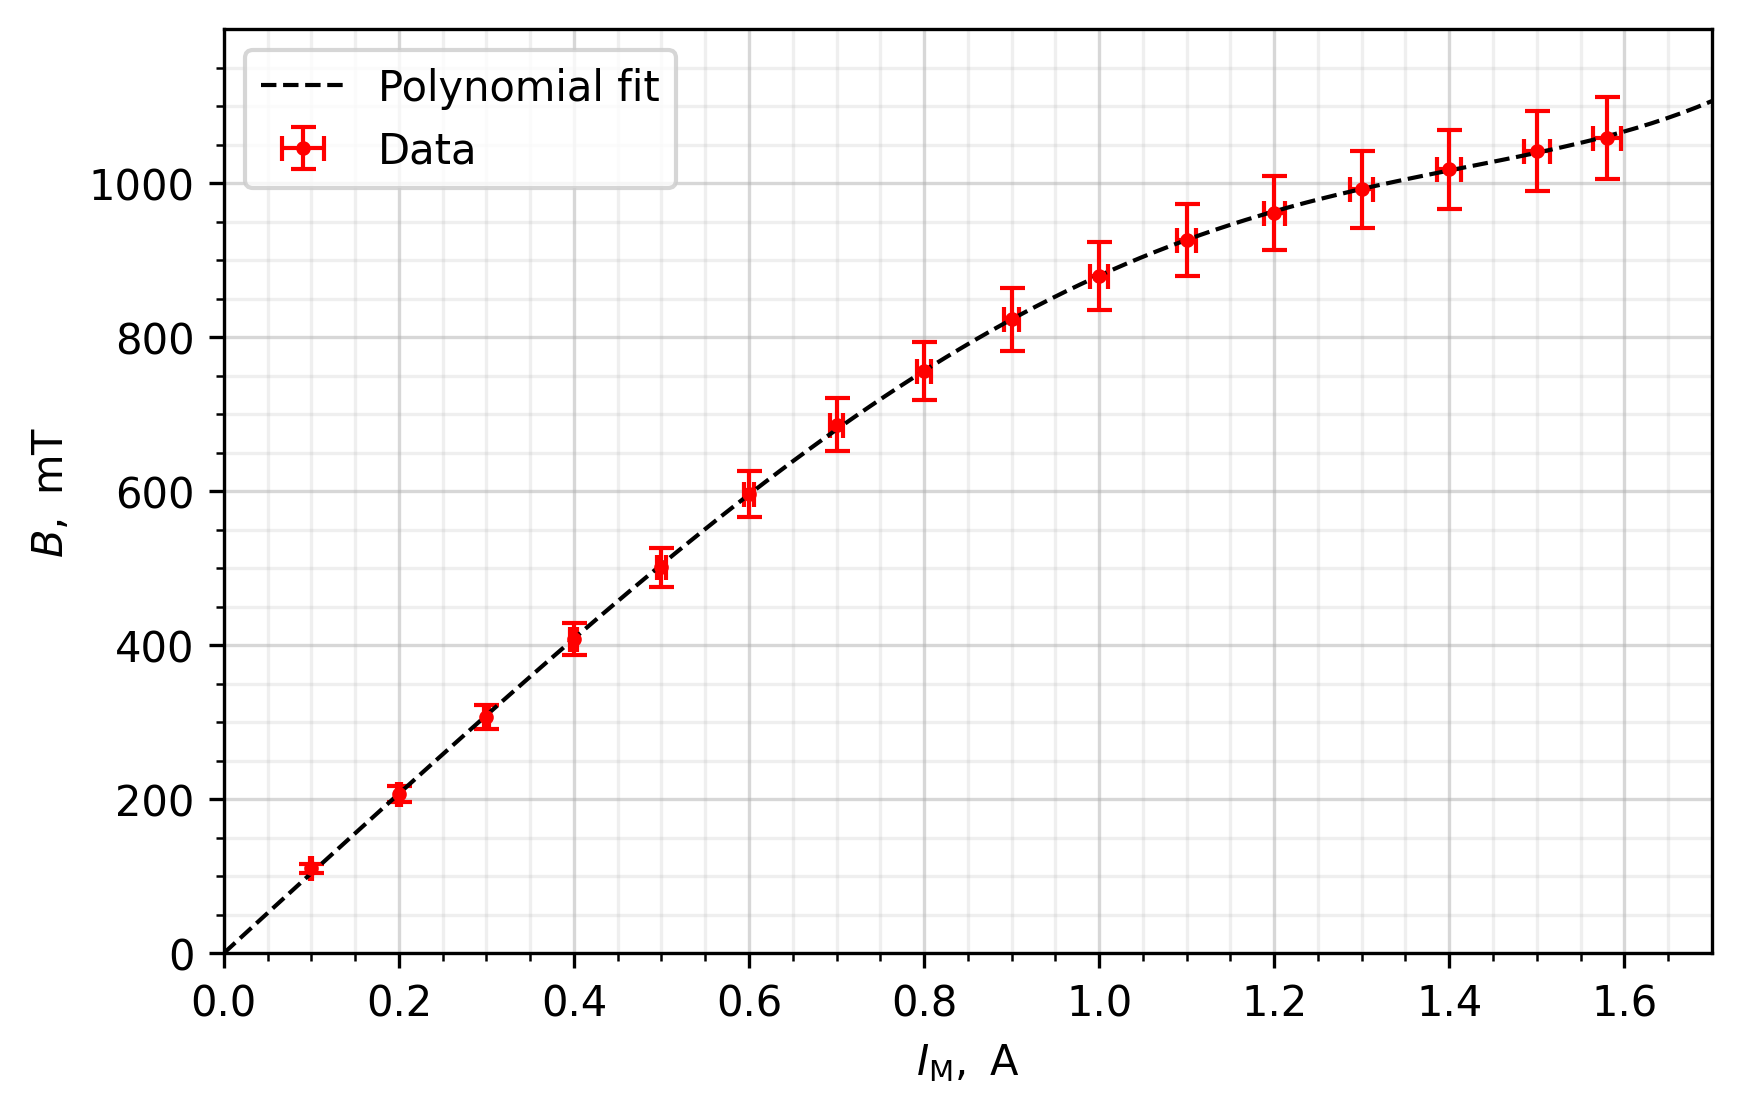
\includegraphics[width=0.6\linewidth]{pics/calibration.png}
  \caption{Градуировочная кривая $B(I)$}
  \label{fig:low_freq}
\end{figure}

Аппроксимируем полученные точки полиномом 4 степени (приведён на рисунке). Хоть и видно что глобально он плохо описывает зависимость
(за пределами самой большой по току точке), интерполирует наши точки он прекрасно.

Для оценки погрешности измерения $B$ возьмём чисто инструментальную погрешность -- ${\varepsilon(B) = 5 \%}$.

\subsection{Измерение ЭДС Холла}
Теперь приведем результаты измерений ЭДС Холла. В табличном виде они находятся в
\textit{табл. \ref{table:hall}} в приложении. Здесь же будет приведён исключительно график зависимости ЭДС Холла от магнитной индукции
с учетом градуировки.
\newpage
\begin{figure}[H]
  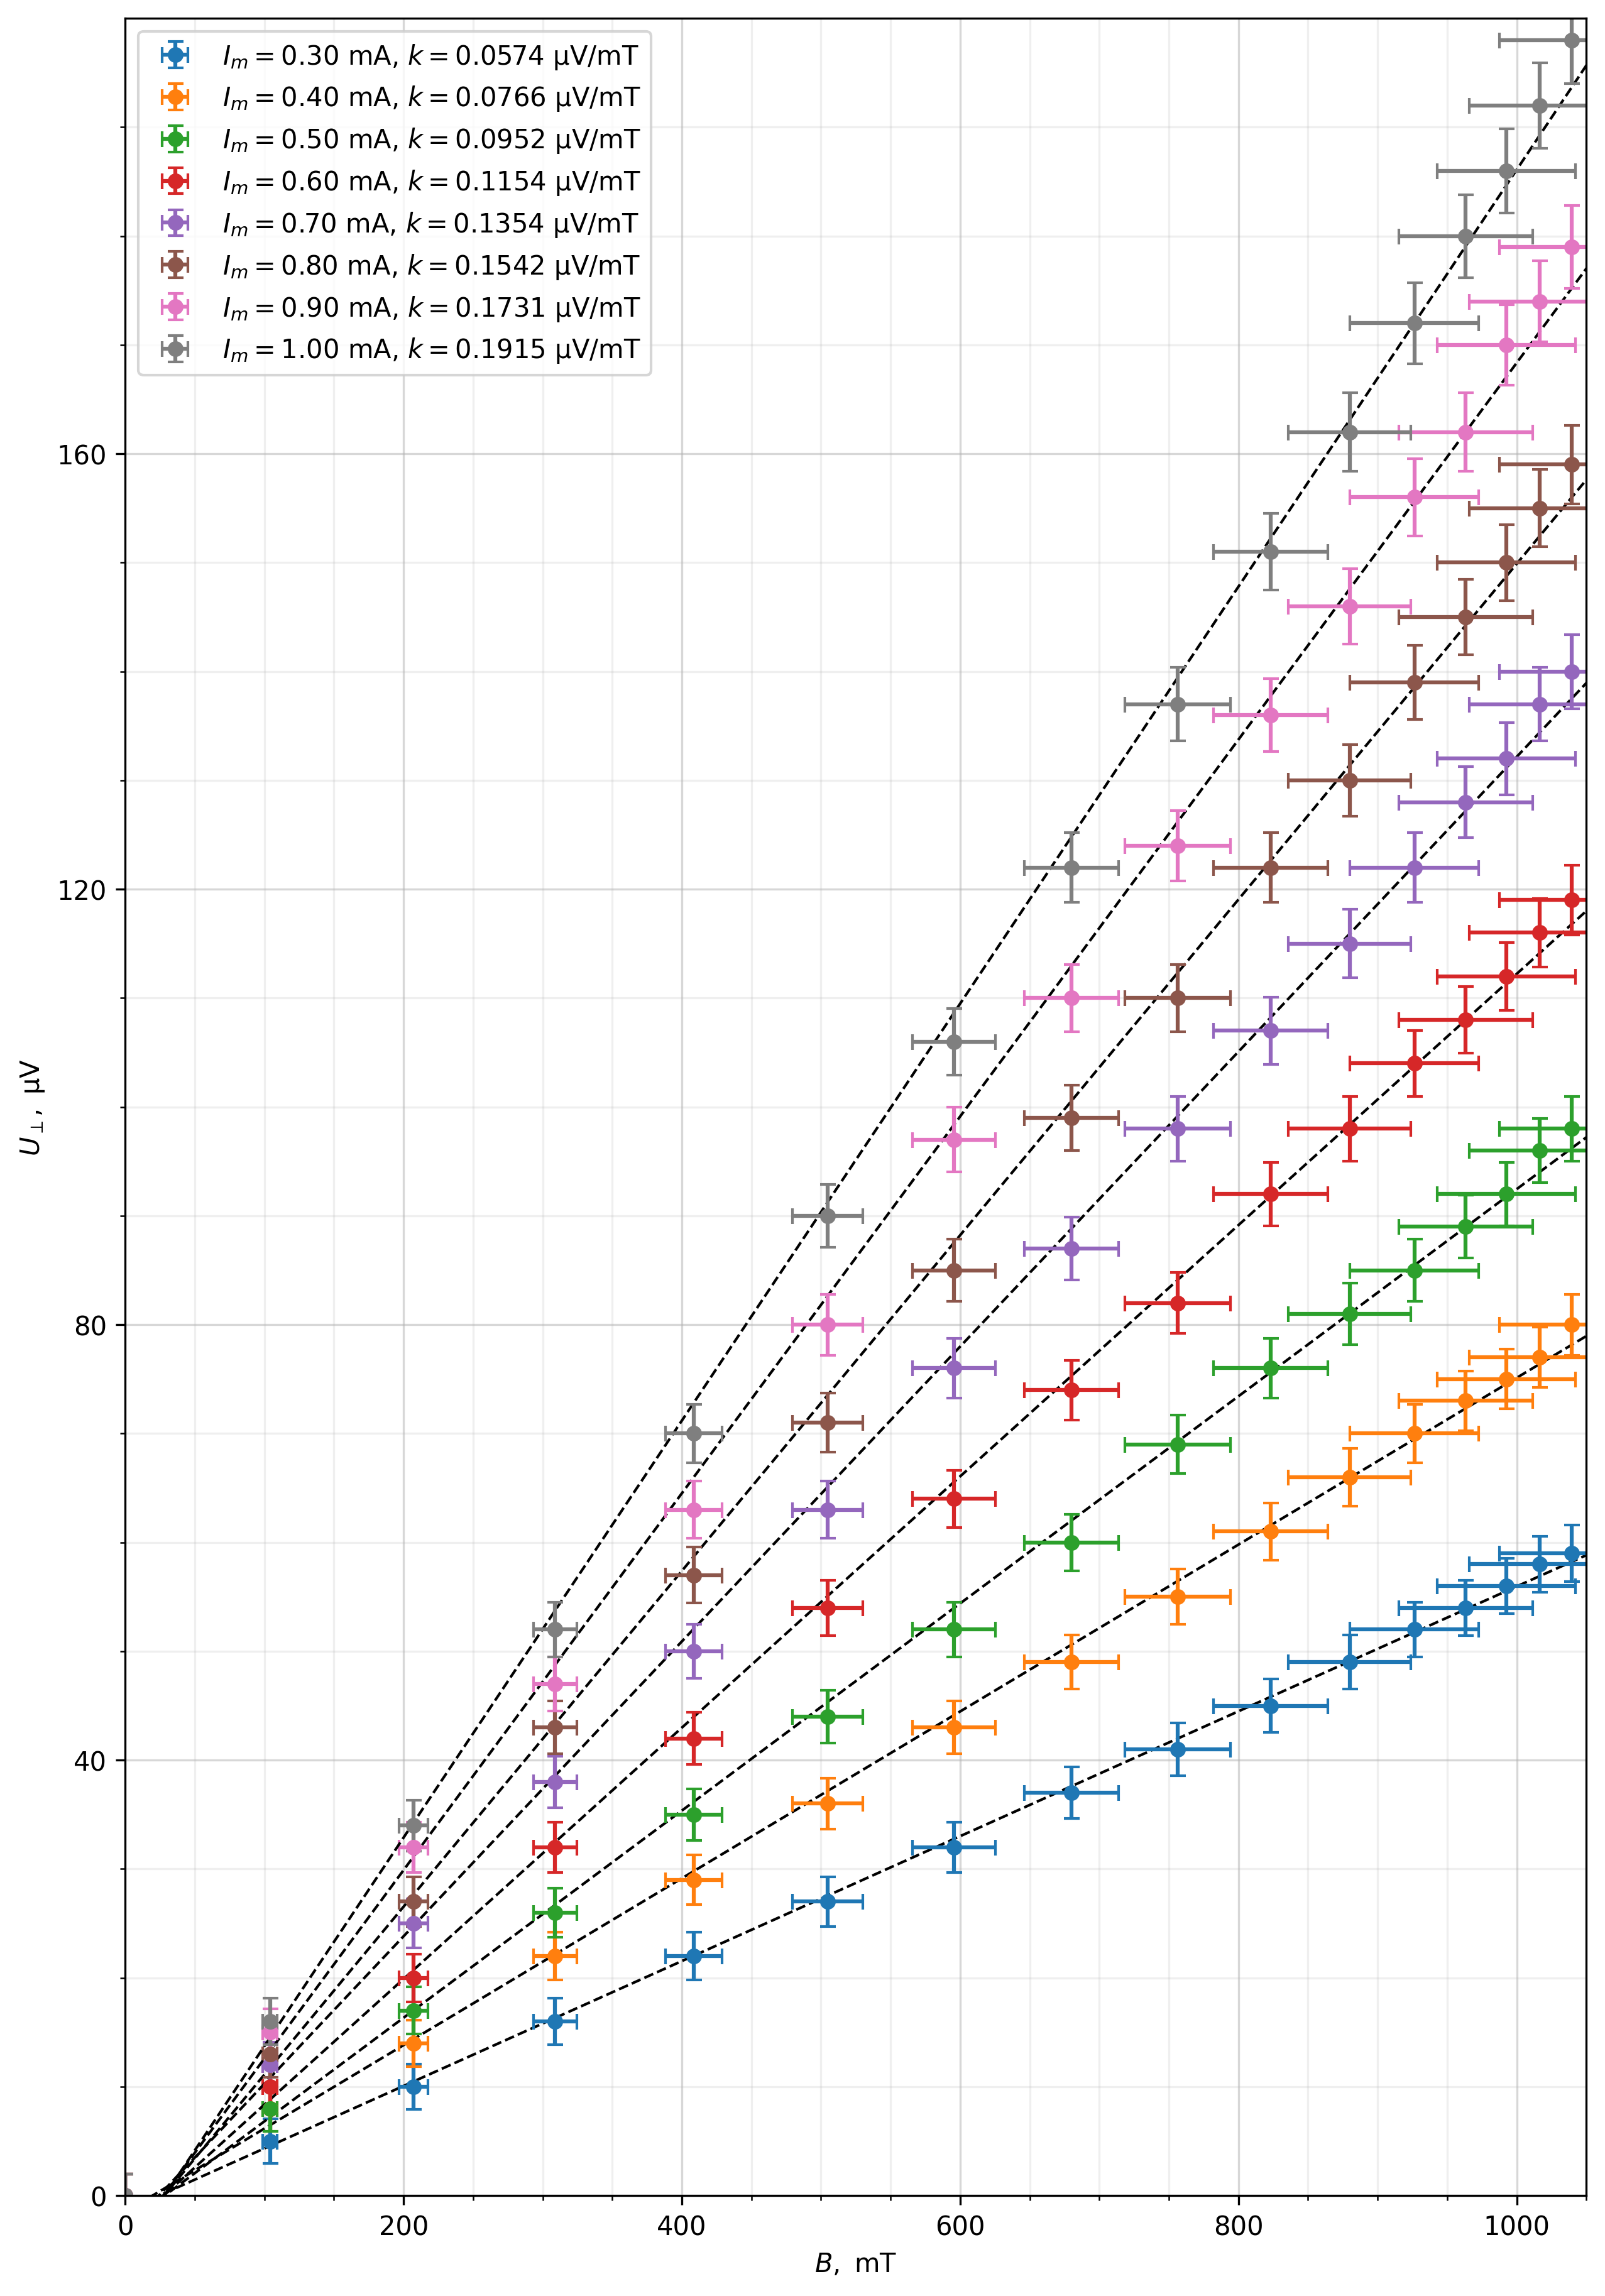
\includegraphics[width=0.95\textwidth]{pics/second_part.png}
  \caption{Зависимость ЭДС Холла от величины магнитной индукции}
\end{figure}
\newpage

Для удобства сведём полученные результаты (угловые коэффициенты) в единую таблицу.
\begin{table}[H]
  \begin{tabular}{|l|c|c|c|c|c|c|c|c|}

    \hline
    $I,~\mathrm{mA}$ & 0.30 & 0.40 & 0.50 & 0.60 & 0.70 & 0.80 & 0.90 & 1.00 \\ \hline
    $k,~\mathrm{mV/T}$ & 0.0574 & 0.0766 & 0.0952 & 0.1154 & 0.1354 & 0.1542 & 0.1731 & 0.1915 \\
    \hline
  \end{tabular}
  \caption{Зависимость крутизны зависимости ЭДС Холла к индукции от полного тока}
\end{table}

\begin{figure}[H]
  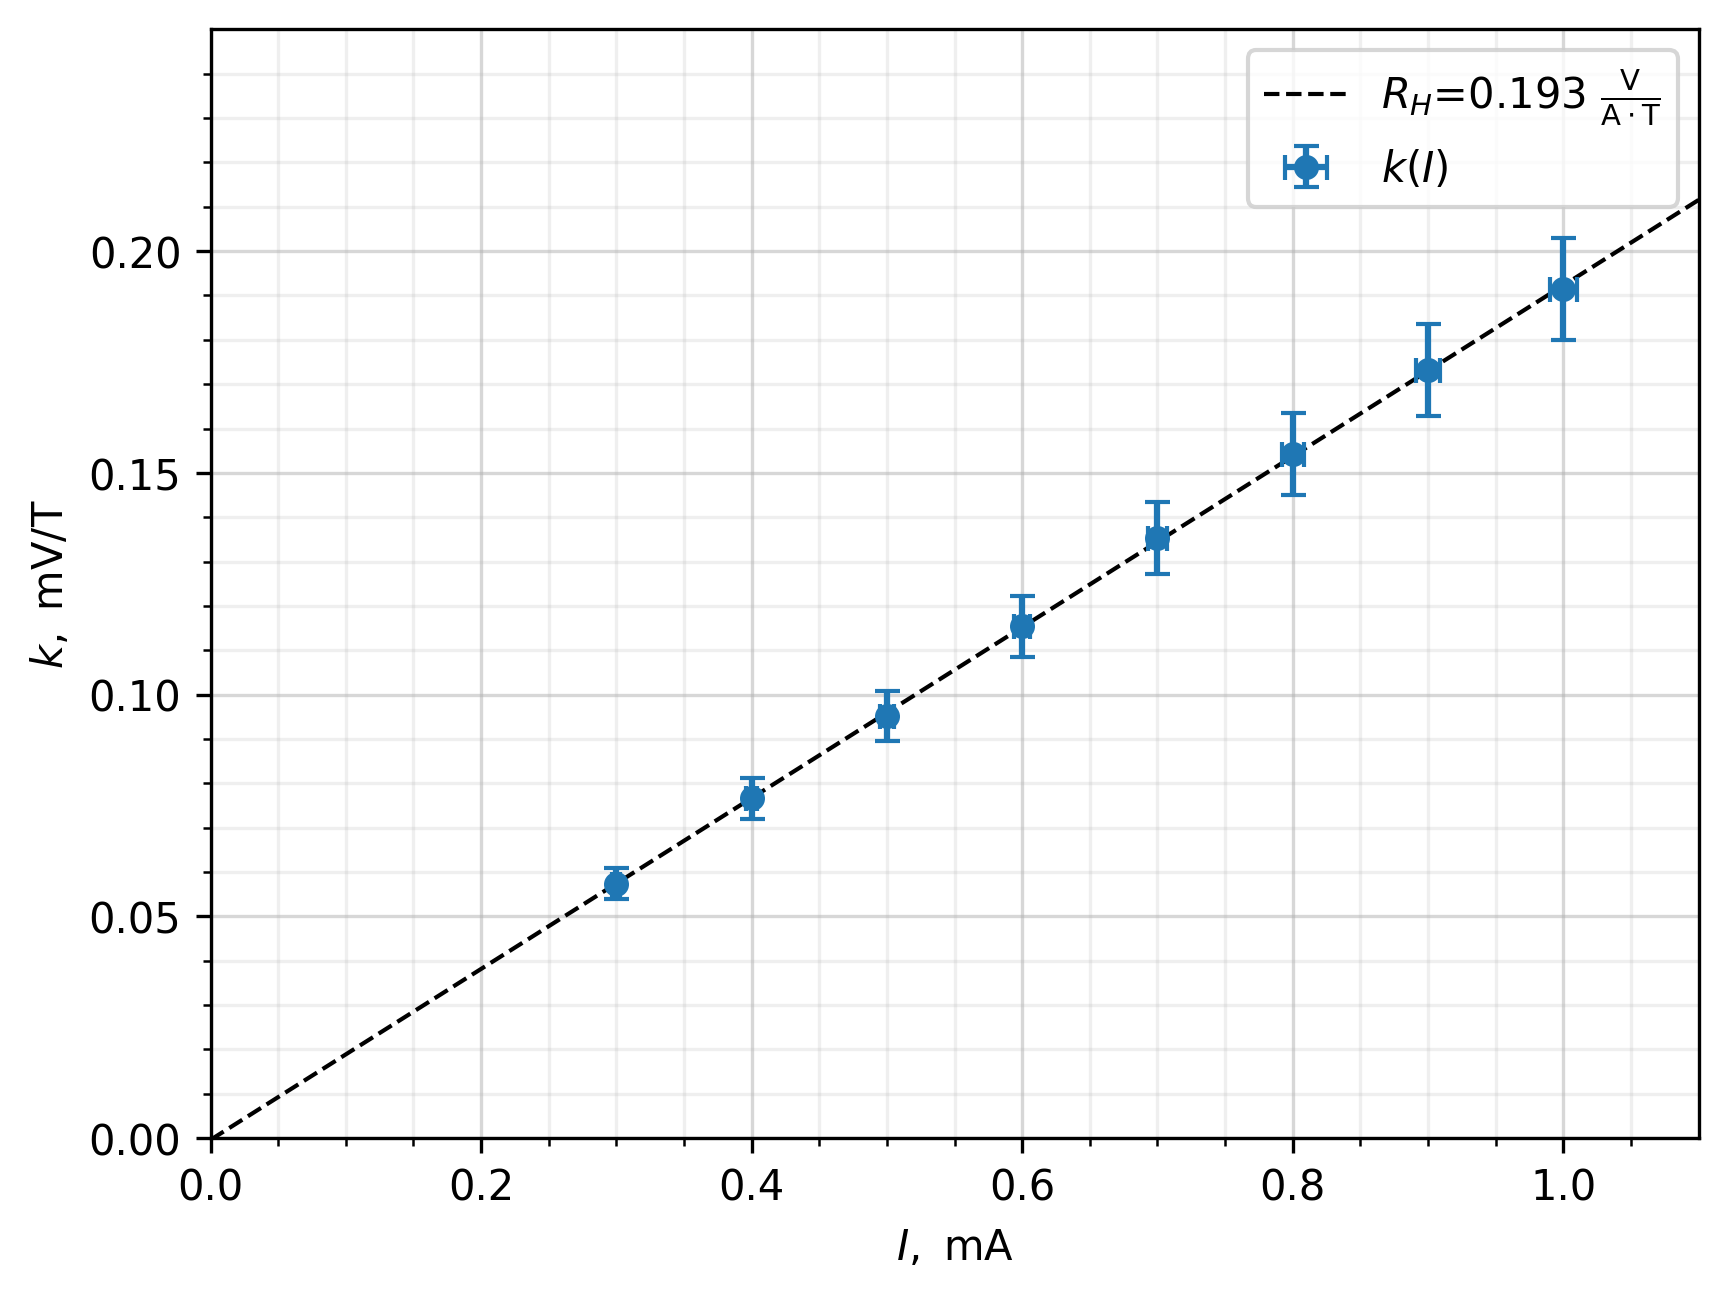
\includegraphics[width=0.75\textwidth]{pics/hallconst.png}
  \caption{Зависимость крутизны зависимости ЭДС Холла от тока через образец}
  \label{fig:hallconst}
\end{figure}

Из \textit{рис. \ref{fig:hallconst}} найдем коэффициент Холла, используя (\ref{eq:uperp}):
\[R_H / a= (0.193\pm 0.011) \mathrm{\dfrac{V}{A\cdot T}}\]
\[R_H = (4.25\pm 0.24)\cdot 10^{-4} \mathrm{\dfrac{V\cdot m}{A\cdot T}}\]

Из (\ref{eq:r_hall}) находим концентрацию носителей заряда:
\[n = \dfrac{1}{R_h \cdot e} = 1.47\cdot 10^{22}~\mathrm{m^{-3}} = 1.47\cdot 10^{16}~\mathrm{cm^{-3}}\]

Зная направление намотки катушки и знак эффекта Холла, понимаем, что германий легирован донорной добавкой (электронная проводимость).

Найдём так же проводимость образца по формуле (\ref{eq:sigma}):
\[\sigma = \frac{100\mA \cdot 3.0~\mathrm{mm}}{1.752\mV\cdot 2.2~\mathrm{mm} \cdot 2.5~\mathrm{mm}} = 31100 ~(\mathrm{\Omega\cdot m})^{-1}\]
а из этого получим подвижность электронов
\[\mu = \sigma/(en) = (13.2\pm 0.8)~\mathrm{m^2/V/s} = (132\pm 8)\cdot10^3~\mathrm{cm^2/V/s}\]

\section{Вывод}
В работе удалось пронаблюдать эффект Холла, определить тип проводимости образца и найти подвижность и концентрацию носителей заряда с хорошей точностью ($\sim 7\%$).
\section{Приложение}


\begin{table}[H]
  \hspace{-4mm}
  \footnotesize
  \begin{tabular}{|ll|ll|ll|ll|ll|ll|ll|ll|}
    \hline
    \multicolumn{2}{|c|}{0.30 mA}                           & \multicolumn{2}{c|}{0.40 mA}                           & \multicolumn{2}{c|}{0.50 mA}                           & \multicolumn{2}{c|}{0.60 mA}                           & \multicolumn{2}{c|}{0.70 mA}                           & \multicolumn{2}{c|}{0.80 mA}                           & \multicolumn{2}{c|}{0.90 mA}                           & \multicolumn{2}{c|}{1.0 mA}                            \\ \hline
    \multicolumn{1}{|r|}{I, A} & \multicolumn{1}{r|}{\parbox{6mm}{\!\!\tiny$U_\perp, \mathrm{\mu V}$}} & \multicolumn{1}{r|}{I, A} & \multicolumn{1}{r|}{\parbox{6mm}{\!\!\tiny$U_\perp, \mathrm{\mu V}$}} & \multicolumn{1}{r|}{I, A} & \multicolumn{1}{r|}{\parbox{6mm}{\!\!\tiny$U_\perp, \mathrm{\mu V}$}} & \multicolumn{1}{r|}{I, A} & \multicolumn{1}{r|}{\parbox{6mm}{\!\!\tiny$U_\perp, \mathrm{\mu V}$}} & \multicolumn{1}{r|}{I, A} & \multicolumn{1}{r|}{\parbox{6mm}{\!\!\tiny$U_\perp, \mathrm{\mu V}$}} & \multicolumn{1}{r|}{I, A} & \multicolumn{1}{r|}{\parbox{6mm}{\!\!\tiny$U_\perp, \mathrm{\mu V}$}} & \multicolumn{1}{r|}{I, A} & \multicolumn{1}{r|}{\parbox{6mm}{\!\!\tiny$U_\perp, \mathrm{\mu V}$}} & \multicolumn{1}{r|}{I, A} & \multicolumn{1}{r|}{\parbox{6mm}{\!\!\tiny$U_\perp, \mathrm{\mu V}$}} \\ \hline
    \multicolumn{1}{|l|}{0.0}  & -7                         & \multicolumn{1}{l|}{0.0}  & -10                        & \multicolumn{1}{l|}{0.0}  & -13                        & \multicolumn{1}{l|}{0.0}  & -17                        & \multicolumn{1}{l|}{0.0}  & -20                        & \multicolumn{1}{l|}{0.0}  & -22                        & \multicolumn{1}{l|}{0.0}  & -25                        & \multicolumn{1}{l|}{0.0}  & -28                        \\ \hline
    \multicolumn{1}{|l|}{0.1}  & -2                         & \multicolumn{1}{l|}{0.1}  & -2                         & \multicolumn{1}{l|}{0.1}  & -5                         & \multicolumn{1}{l|}{0.1}  & -7                         & \multicolumn{1}{l|}{0.1}  & -8                         & \multicolumn{1}{l|}{0.1}  & -9                         & \multicolumn{1}{l|}{0.1}  & -10                        & \multicolumn{1}{l|}{0.1}  & -12                        \\ \hline
    \multicolumn{1}{|l|}{0.2}  & 3                          & \multicolumn{1}{l|}{0.2}  & 4                          & \multicolumn{1}{l|}{0.2}  & 4                          & \multicolumn{1}{l|}{0.2}  & 3                          & \multicolumn{1}{l|}{0.2}  & 5                          & \multicolumn{1}{l|}{0.2}  & 5                          & \multicolumn{1}{l|}{0.2}  & 7                          & \multicolumn{1}{l|}{0.2}  & 6                          \\ \hline
    \multicolumn{1}{|l|}{0.3}  & 9                          & \multicolumn{1}{l|}{0.3}  & 12                         & \multicolumn{1}{l|}{0.3}  & 13                         & \multicolumn{1}{l|}{0.3}  & 15                         & \multicolumn{1}{l|}{0.3}  & 18                         & \multicolumn{1}{l|}{0.3}  & 21                         & \multicolumn{1}{l|}{0.3}  & 22                         & \multicolumn{1}{l|}{0.3}  & 24                         \\ \hline
    \multicolumn{1}{|l|}{0.4}  & 15                         & \multicolumn{1}{l|}{0.4}  & 19                         & \multicolumn{1}{l|}{0.4}  & 22                         & \multicolumn{1}{l|}{0.4}  & 25                         & \multicolumn{1}{l|}{0.4}  & 30                         & \multicolumn{1}{l|}{0.4}  & 35                         & \multicolumn{1}{l|}{0.4}  & 38                         & \multicolumn{1}{l|}{0.4}  & 42                         \\ \hline
    \multicolumn{1}{|l|}{0.5}  & 20                         & \multicolumn{1}{l|}{0.5}  & 26                         & \multicolumn{1}{l|}{0.5}  & 31                         & \multicolumn{1}{l|}{0.5}  & 37                         & \multicolumn{1}{l|}{0.5}  & 43                         & \multicolumn{1}{l|}{0.5}  & 49                         & \multicolumn{1}{l|}{0.5}  & 55                         & \multicolumn{1}{l|}{0.5}  & 62                         \\ \hline
    \multicolumn{1}{|l|}{0.6}  & 25                         & \multicolumn{1}{l|}{0.6}  & 33                         & \multicolumn{1}{l|}{0.6}  & 39                         & \multicolumn{1}{l|}{0.6}  & 47                         & \multicolumn{1}{l|}{0.6}  & 56                         & \multicolumn{1}{l|}{0.6}  & 63                         & \multicolumn{1}{l|}{0.6}  & 72                         & \multicolumn{1}{l|}{0.6}  & 78                         \\ \hline
    \multicolumn{1}{|l|}{0.7}  & 30                         & \multicolumn{1}{l|}{0.7}  & 39                         & \multicolumn{1}{l|}{0.7}  & 47                         & \multicolumn{1}{l|}{0.7}  & 57                         & \multicolumn{1}{l|}{0.7}  & 67                         & \multicolumn{1}{l|}{0.7}  & 77                         & \multicolumn{1}{l|}{0.7}  & 85                         & \multicolumn{1}{l|}{0.7}  & 94                         \\ \hline
    \multicolumn{1}{|l|}{0.8}  & 34                         & \multicolumn{1}{l|}{0.8}  & 45                         & \multicolumn{1}{l|}{0.8}  & 56                         & \multicolumn{1}{l|}{0.8}  & 65                         & \multicolumn{1}{l|}{0.8}  & 78                         & \multicolumn{1}{l|}{0.8}  & 88                         & \multicolumn{1}{l|}{0.8}  & 99                         & \multicolumn{1}{l|}{0.8}  & 109                        \\ \hline
    \multicolumn{1}{|l|}{0.9}  & 38                         & \multicolumn{1}{l|}{0.9}  & 51                         & \multicolumn{1}{l|}{0.9}  & 63                         & \multicolumn{1}{l|}{0.9}  & 75                         & \multicolumn{1}{l|}{0.9}  & 87                         & \multicolumn{1}{l|}{0.9}  & 100                        & \multicolumn{1}{l|}{0.9}  & 111                        & \multicolumn{1}{l|}{0.9}  & 123                        \\ \hline
    \multicolumn{1}{|l|}{1.0}  & 42                         & \multicolumn{1}{l|}{1.0}  & 56                         & \multicolumn{1}{l|}{1.0}  & 68                         & \multicolumn{1}{l|}{1.0}  & 81                         & \multicolumn{1}{l|}{1.0}  & 95                         & \multicolumn{1}{l|}{1.0}  & 108                        & \multicolumn{1}{l|}{1.0}  & 121                        & \multicolumn{1}{l|}{1.0}  & 134                        \\ \hline
    \multicolumn{1}{|l|}{1.1}  & 45                         & \multicolumn{1}{l|}{1.1}  & 60                         & \multicolumn{1}{l|}{1.1}  & 72                         & \multicolumn{1}{l|}{1.1}  & 87                         & \multicolumn{1}{l|}{1.1}  & 102                        & \multicolumn{1}{l|}{1.1}  & 117                        & \multicolumn{1}{l|}{1.1}  & 131                        & \multicolumn{1}{l|}{1.1}  & 144                        \\ \hline
    \multicolumn{1}{|l|}{1.2}  & 47                         & \multicolumn{1}{l|}{1.2}  & 63                         & \multicolumn{1}{l|}{1.2}  & 76                         & \multicolumn{1}{l|}{1.2}  & 91                         & \multicolumn{1}{l|}{1.2}  & 108                        & \multicolumn{1}{l|}{1.2}  & 123                        & \multicolumn{1}{l|}{1.2}  & 137                        & \multicolumn{1}{l|}{1.2}  & 152                        \\ \hline
    \multicolumn{1}{|l|}{1.3}  & 49                         & \multicolumn{1}{l|}{1.3}  & 65                         & \multicolumn{1}{l|}{1.3}  & 79                         & \multicolumn{1}{l|}{1.3}  & 95                         & \multicolumn{1}{l|}{1.3}  & 112                        & \multicolumn{1}{l|}{1.3}  & 128                        & \multicolumn{1}{l|}{1.3}  & 145                        & \multicolumn{1}{l|}{1.3}  & 158                        \\ \hline
    \multicolumn{1}{|l|}{1.4}  & 51                         & \multicolumn{1}{l|}{1.4}  & 67                         & \multicolumn{1}{l|}{1.4}  & 83                         & \multicolumn{1}{l|}{1.4}  & 99                         & \multicolumn{1}{l|}{1.4}  & 117                        & \multicolumn{1}{l|}{1.4}  & 133                        & \multicolumn{1}{l|}{1.4}  & 149                        & \multicolumn{1}{l|}{1.4}  & 164                        \\ \hline
    \multicolumn{1}{|l|}{1.5}  & 52                         & \multicolumn{1}{l|}{1.5}  & 70                         & \multicolumn{1}{l|}{1.5}  & 85                         & \multicolumn{1}{l|}{1.5}  & 102                        & \multicolumn{1}{l|}{1.5}  & 120                        & \multicolumn{1}{l|}{1.5}  & 137                        & \multicolumn{1}{l|}{1.5}  & 154                        & \multicolumn{1}{l|}{1.5}  & 170                        \\ \hline
  \end{tabular}
  \caption{Результаты измерения для 2 пункта}
  \label{table:hall}
\end{table}

\end{document}
